% \textbf{Định lý Earnshaw và thấu kính tĩnh điện}

% Một vòng dây điện tích \(Q\) hình đa giác đều \(n\) cạnh có bán kính đường tròn ngoại tiếp \(R\). Trục \(\Delta\) là trục đi qua tâm và vuông góc với mặt phẳng vòng dây có dạng đối xứng trụ.

% \ \ 

% \textbf{1.} Chứng minh rằng, điện trường ở gần trục \(\Delta\).

% \ \ 

% \textbf{2.} Tính vector điện trường \(\mathbf{E}\) tại một vị trí gần trục \(\Delta\).

% \ \ 

% Theo định lý Earnshaw, một hệ điện tích trong chân không không thể tạo ra một điểm cân bằng bền chỉ bởi các tương tác tĩnh điện.

% \ \  

% \textbf{3.} Chỉ ra rằng trong bài toán này, vị trí cân bằng không thể là vị trí cân bằng bền với mọi chuyển động.

% \ \ 

% \textbf{4.} Bắn một hạt điện tích \(q\) khối lượng \(m\) với vận tốc \(v_0\) song song với trục \(\Delta\) và cách trục \(\Delta\) một khoảng \(b\) (với \(b \ll R\) ). Quỹ đạo của hạt điện tích đi qua vòng dây điện tích giống như một tia sáng đi qua thấu kính có tiêu cự \(f\). Tính tiêu cự \(f\) này theo \(n\), \(R\), \(Q\), \(q\), \(\varepsilon_0\), \(m\) và \(v_0\).

\textbf{Hiệu ứng bề mặt} \footnote{Skin effect.}

Hiệu ứng bề mặt là một hiệu ứng xuất hiện phổ biến trong các các đường mạch điện truyền dẫn dòng điện cao tần. Theo đó, thay vì phân bố đều trên toàn dây dẫn như các dòng điện tần số thấp, ở tần số cao, các dòng điện tập trung chủ yếu ở sát bề mặt kim loại và nhanh chóng giảm theo độ sâu với cấp số mũ.

\ \

\textbf{1. Mô hình mạch tương đương đơn giản}

Quy luật chuyển động của dòng điện trong một vật dẫn với hằng số điện môi \(\mu\) và điện trở suất \(\rho\) có thể được mô tả bởi một mạch điện tương đương (như hình \ref{fig:Equivalent_circuit_skin_effect}) \footnote{Điện kháng \(L_0\) được sử dụng để mô tả hằng số từ thẩm trong chân không \(\mu_0\) của môi trường ngoài. Ta không cần quan tâm đến nó trong bài toán này}. Ở hình \ref{fig:Equivalent_circuit_skin_effect}A, phân bố dòng điện trong tấm vật liệu được tương đương như một mạch điện vô hạn, theo đó, từng khối chữ nhật có chiều dài \(l\), chiều rộng \(w\) và độ dày \(\Delta z\) (như hình \ref{fig:Conductor}) được tương đương như một mắt mạch tương đương gồm một thành phần cảm kháng \(\Delta L\) và một phần điện dẫn \footnote{Nghịch đảo của điện trở.} \( \Delta G \).

\begin{figure}[!h]
    \centering
    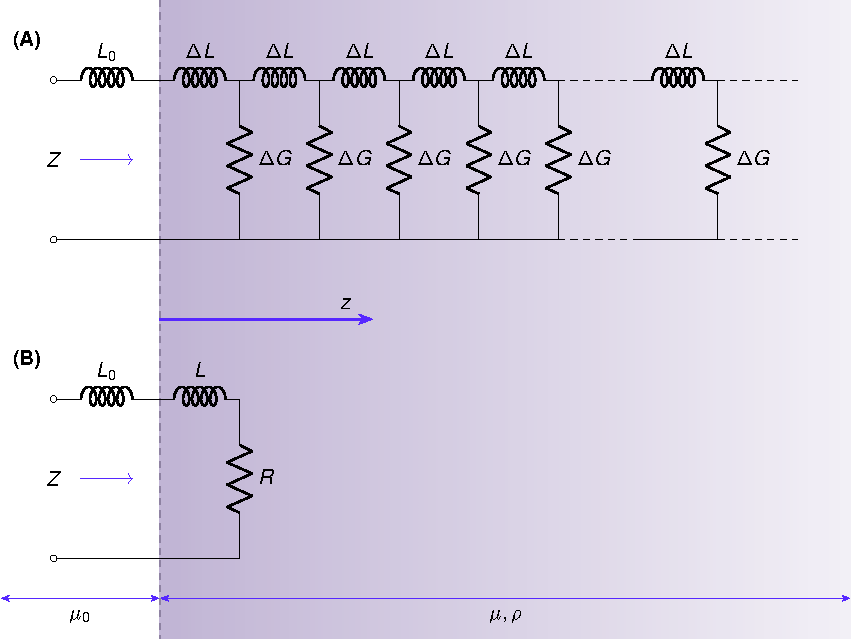
\includegraphics[width=0.9\textwidth]{Problem_3/Figs_P3/Equivalent_circuit_skin_effect.pdf}
    \caption{Mô hình mạch tương đương của hiệu ứng bề mặt. (A) Mạch tương đương phân bố vô hạn trong không gian. (B) Mạch tương đương trở kháng của mạch.}
    \label{fig:Equivalent_circuit_skin_effect}
\end{figure}

Dựa vào các tính toán mạch tương đương, mạng mạch vô hạn tuần hoàn trên có trở kháng quan sát từ phía bề mặt ngăn cách hai môi trường là \(Z\) và có thể được phân tích như tổng của hai phân tử \(R\) và \(L\) (như hình \ref{fig:Equivalent_circuit_skin_effect}B).

\begin{figure}
    \centering
    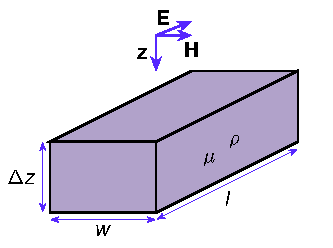
\includegraphics[width=0.6\textwidth]{Problem_3/Figs_P3/Conductor.pdf}
    \caption{Mô hình một phần tử trong khối vật dẫn.}
    \label{fig:Conductor}
\end{figure}

\textbf{Câu hỏi a.} Tìm \( \Delta L \) và \( \Delta G \) của mạch trong mô hình mạch tương đương vô hạn theo \(\mu\), \(\rho\), \(w\), \(l\) và \( \Delta z \).

\ \

\textbf{Câu hỏi b.} Tìm các thông số trở kháng \(Z\), \(R\) và \(L\) theo \(\mu\), \(\rho\), \(w\), \(l\) và tần số \(\omega\) của dòng điện.

\ \

\textbf{Câu hỏi c.} Độ sâu bề mặt\footnote{Skin depth.} là độ sâu để biên độ dòng điện giảm đi \(e\) lần. Xác định độ sâu bề mặt của tấm vật liệu theo tần số \(\omega\) của dòng điện, độ từ thẩm \(\mu\) và điện trở suất \(\rho\).

\ \

\textbf{2. Điện trở gây bởi hiệu ứng bề mặt}

\ \

\textbf{Câu hỏi d.} Chứng minh rằng, ta có thể tính điện trở \(R\) tương đương của một đoạn vật dẫn điện chịu ảnh hưởng bởi hiệu ứng bề mặt có thể tính theo công thức:
\begin{equation}
    R = \dfrac{1}{\mu_0} \dfrac{\partial L_0}{\partial z} R_S,
\end{equation}
trong đó
\begin{itemize}
    \item \(L_0\) là độ tự cảm của một miếng bề mặt vật dẫn được xét với giả thiết độ sâu bề mặt bằng không.
    \item Tọa độ \(z\) được hiểu là tọa độ có trục vuông góc với bề mặt.
    \item \(R_S = \sqrt{\omega \mu \rho/2}\) được gọi là hệ số điện trở suất bề mặt.
\end{itemize}

\ \

\textbf{Câu hỏi e.} Tính điện trở gây ra bởi hiệu ứng bề mặt đối với hai ống dây dẫn tròn có chiều dài \(l\), bán kính \(a\) và có trục dây đặt cách nhau một khoảng \(2b\).